\documentclass{standalone}
\usepackage{tikz}
\usetikzlibrary{patterns, positioning}


\begin{document}
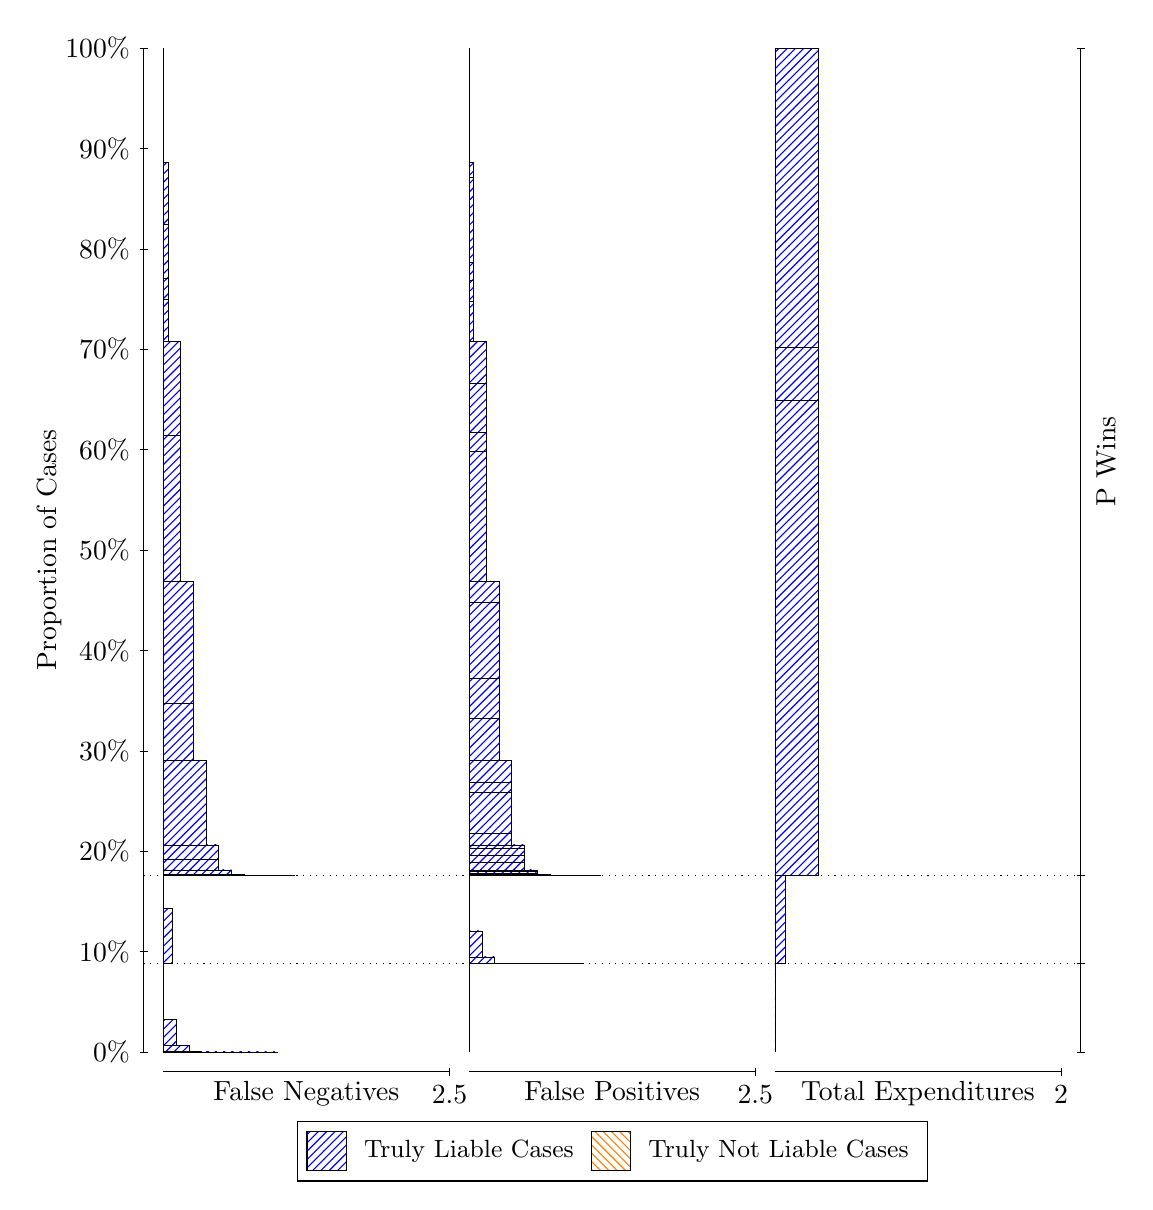
\begin{tikzpicture}
\draw[black, very thin] (1.5,1.75) -- (1.5,14.5);
\node[rotate=90, text=black, anchor=center] at (0.3, 8.125) {Proportion of Cases};
\draw[black, very thin] (1.45,1.75) -- (1.55,1.75);
\node[text=black, anchor=east] at (1.45, 1.75) {0\%};
\draw[black, very thin] (1.45,3.025) -- (1.55,3.025);
\node[text=black, anchor=east] at (1.45, 3.025) {10\%};
\draw[black, very thin] (1.45,4.3) -- (1.55,4.3);
\node[text=black, anchor=east] at (1.45, 4.3) {20\%};
\draw[black, very thin] (1.45,5.575) -- (1.55,5.575);
\node[text=black, anchor=east] at (1.45, 5.575) {30\%};
\draw[black, very thin] (1.45,6.85) -- (1.55,6.85);
\node[text=black, anchor=east] at (1.45, 6.85) {40\%};
\draw[black, very thin] (1.45,8.125) -- (1.55,8.125);
\node[text=black, anchor=east] at (1.45, 8.125) {50\%};
\draw[black, very thin] (1.45,9.4) -- (1.55,9.4);
\node[text=black, anchor=east] at (1.45, 9.4) {60\%};
\draw[black, very thin] (1.45,10.675) -- (1.55,10.675);
\node[text=black, anchor=east] at (1.45, 10.675) {70\%};
\draw[black, very thin] (1.45,11.95) -- (1.55,11.95);
\node[text=black, anchor=east] at (1.45, 11.95) {80\%};
\draw[black, very thin] (1.45,13.225) -- (1.55,13.225);
\node[text=black, anchor=east] at (1.45, 13.225) {90\%};
\draw[black, very thin] (1.45,14.5) -- (1.55,14.5);
\node[text=black, anchor=east] at (1.45, 14.5) {100\%};

\draw[black, very thin] (13.4,1.75) -- (13.4,14.5);
\draw[black, very thin] (13.35,1.75) -- (13.45,1.75);
\node[anchor=west] at (13.35, 1.75) {};
\draw[black, very thin] (13.35,2.872) -- (13.45,2.872);
\node[anchor=west] at (13.35, 2.872) {};
\draw[black, very thin] (13.35,3.9941) -- (13.45,3.9941);
\node[anchor=west] at (13.35, 3.9941) {};
\draw[black, very thin] (13.35,14.5) -- (13.45,14.5);
\node[anchor=west] at (13.35, 14.5) {};

\draw[black, very thin, pattern color=blue, pattern=north east lines] (1.75,1.75) rectangle (3.2033,1.75);
\draw[black, very thin, pattern color=blue, pattern=north east lines] (1.75,1.75) rectangle (3.0419,1.75);
\draw[black, very thin, pattern color=blue, pattern=north east lines] (1.75,1.75) rectangle (2.8804,1.75);
\draw[black, very thin, pattern color=blue, pattern=north east lines] (1.75,1.75) rectangle (2.7189,1.75);
\draw[black, very thin, pattern color=blue, pattern=north east lines] (1.75,1.75) rectangle (2.5574,1.75);
\draw[black, very thin, pattern color=blue, pattern=north east lines] (1.75,1.75) rectangle (2.3959,1.7503);
\draw[black, very thin, pattern color=blue, pattern=north east lines] (1.75,1.7503) rectangle (2.2344,1.7579);
\draw[black, very thin, pattern color=blue, pattern=north east lines] (1.75,1.7579) rectangle (2.073,1.8357);
\draw[black, very thin, pattern color=blue, pattern=north east lines] (1.75,1.8357) rectangle (1.9115,2.1659);
\draw[black, very thin, pattern color=orange, pattern=north west lines] (1.75,2.1659) rectangle (1.75,2.1659);
\draw[black, very thin, pattern color=blue, pattern=north east lines] (1.75,2.1659) rectangle (1.75,2.872);
\draw[black, very thin, pattern color=blue, pattern=north east lines] (1.75,2.872) rectangle (1.859,3.5781);
\draw[black, very thin, pattern color=orange, pattern=north west lines] (1.75,3.5781) rectangle (1.75,3.5781);
\draw[black, very thin, pattern color=blue, pattern=north east lines] (1.75,3.5781) rectangle (1.75,3.9941);
\draw[black, very thin, pattern color=blue, pattern=north east lines] (1.75,3.9941) rectangle (3.4213,3.9941);
\draw[black, very thin, pattern color=blue, pattern=north east lines] (1.75,3.9941) rectangle (3.2599,3.9941);
\draw[black, very thin, pattern color=blue, pattern=north east lines] (1.75,3.9941) rectangle (3.2599,3.9941);
\draw[black, very thin, pattern color=blue, pattern=north east lines] (1.75,3.9941) rectangle (3.0984,3.9941);
\draw[black, very thin, pattern color=blue, pattern=north east lines] (1.75,3.9941) rectangle (3.0984,3.9941);
\draw[black, very thin, pattern color=blue, pattern=north east lines] (1.75,3.9941) rectangle (2.9369,3.9946);
\draw[black, very thin, pattern color=blue, pattern=north east lines] (1.75,3.9946) rectangle (2.7754,3.9988);
\draw[black, very thin, pattern color=blue, pattern=north east lines] (1.75,3.9988) rectangle (2.7754,4.0018);
\draw[black, very thin, pattern color=blue, pattern=north east lines] (1.75,4.0018) rectangle (2.6139,4.062);
\draw[black, very thin, pattern color=blue, pattern=north east lines] (1.75,4.062) rectangle (2.4524,4.1925);
\draw[black, very thin, pattern color=blue, pattern=north east lines] (1.75,4.1925) rectangle (2.4524,4.3808);
\draw[black, very thin, pattern color=blue, pattern=north east lines] (1.75,4.3808) rectangle (2.291,5.451);
\draw[black, very thin, pattern color=blue, pattern=north east lines] (1.75,5.451) rectangle (2.1295,6.1753);
\draw[black, very thin, pattern color=blue, pattern=north east lines] (1.75,6.1753) rectangle (2.1295,7.7224);
\draw[black, very thin, pattern color=blue, pattern=north east lines] (1.75,7.7224) rectangle (1.968,9.5804);
\draw[black, very thin, pattern color=blue, pattern=north east lines] (1.75,9.5804) rectangle (1.968,10.772);
\draw[black, very thin, pattern color=blue, pattern=north east lines] (1.75,10.772) rectangle (1.8065,11.306);
\draw[black, very thin, pattern color=blue, pattern=north east lines] (1.75,11.306) rectangle (1.8065,11.576);
\draw[black, very thin, pattern color=blue, pattern=north east lines] (1.75,11.576) rectangle (1.8065,12.268);
\draw[black, very thin, pattern color=blue, pattern=north east lines] (1.75,12.268) rectangle (1.8065,13.043);
\draw[black, very thin, pattern color=orange, pattern=north west lines] (1.75,13.043) rectangle (1.75,13.043);
\draw[black, very thin, pattern color=blue, pattern=north east lines] (1.75,13.043) rectangle (1.75,14.5);
\draw[black, very thin, pattern color=orange, pattern=north west lines] (5.6333,1.75) rectangle (5.6333,1.75);
\draw[black, very thin, pattern color=blue, pattern=north east lines] (5.6333,1.75) rectangle (5.6333,2.872);
\draw[black, very thin, pattern color=orange, pattern=north west lines] (5.6333,2.872) rectangle (7.0867,2.872);
\draw[black, very thin, pattern color=blue, pattern=north east lines] (5.6333,2.872) rectangle (7.0867,2.872);
\draw[black, very thin, pattern color=blue, pattern=north east lines] (5.6333,2.872) rectangle (6.9252,2.872);
\draw[black, very thin, pattern color=blue, pattern=north east lines] (5.6333,2.872) rectangle (6.7637,2.872);
\draw[black, very thin, pattern color=blue, pattern=north east lines] (5.6333,2.872) rectangle (6.6022,2.872);
\draw[black, very thin, pattern color=blue, pattern=north east lines] (5.6333,2.872) rectangle (6.4407,2.872);
\draw[black, very thin, pattern color=blue, pattern=north east lines] (5.6333,2.872) rectangle (6.2793,2.8723);
\draw[black, very thin, pattern color=blue, pattern=north east lines] (5.6333,2.8723) rectangle (6.1178,2.8799);
\draw[black, very thin, pattern color=blue, pattern=north east lines] (5.6333,2.8799) rectangle (5.9563,2.9577);
\draw[black, very thin, pattern color=blue, pattern=north east lines] (5.6333,2.9577) rectangle (5.7948,3.288);
\draw[black, very thin, pattern color=blue, pattern=north east lines] (5.6333,3.288) rectangle (5.6333,3.9941);
\draw[black, very thin, pattern color=orange, pattern=north west lines] (5.6333,3.9941) rectangle (7.3047,3.9941);
\draw[black, very thin, pattern color=blue, pattern=north east lines] (5.6333,3.9941) rectangle (7.3047,3.9941);
\draw[black, very thin, pattern color=orange, pattern=north west lines] (5.6333,3.9941) rectangle (7.1432,3.9941);
\draw[black, very thin, pattern color=blue, pattern=north east lines] (5.6333,3.9941) rectangle (7.1432,3.9941);
\draw[black, very thin, pattern color=orange, pattern=north west lines] (5.6333,3.9941) rectangle (6.9817,3.9941);
\draw[black, very thin, pattern color=blue, pattern=north east lines] (5.6333,3.9941) rectangle (6.9817,3.9941);
\draw[black, very thin, pattern color=blue, pattern=north east lines] (5.6333,3.9941) rectangle (6.9817,3.9941);
\draw[black, very thin, pattern color=blue, pattern=north east lines] (5.6333,3.9941) rectangle (6.9817,3.9941);
\draw[black, very thin, pattern color=orange, pattern=north west lines] (5.6333,3.9941) rectangle (6.8202,3.9941);
\draw[black, very thin, pattern color=blue, pattern=north east lines] (5.6333,3.9941) rectangle (6.8202,3.9945);
\draw[black, very thin, pattern color=blue, pattern=north east lines] (5.6333,3.9945) rectangle (6.8202,3.9946);
\draw[black, very thin, pattern color=orange, pattern=north west lines] (5.6333,3.9946) rectangle (6.6587,3.9946);
\draw[black, very thin, pattern color=blue, pattern=north east lines] (5.6333,3.9946) rectangle (6.6587,3.9973);
\draw[black, very thin, pattern color=blue, pattern=north east lines] (5.6333,3.9973) rectangle (6.6587,4.0018);
\draw[black, very thin, pattern color=blue, pattern=north east lines] (5.6333,4.0018) rectangle (6.4973,4.0221);
\draw[black, very thin, pattern color=orange, pattern=north west lines] (5.6333,4.0221) rectangle (6.4973,4.0221);
\draw[black, very thin, pattern color=blue, pattern=north east lines] (5.6333,4.0221) rectangle (6.4973,4.0404);
\draw[black, very thin, pattern color=blue, pattern=north east lines] (5.6333,4.0404) rectangle (6.4973,4.062);
\draw[black, very thin, pattern color=blue, pattern=north east lines] (5.6333,4.062) rectangle (6.3358,4.1582);
\draw[black, very thin, pattern color=blue, pattern=north east lines] (5.6333,4.1582) rectangle (6.3358,4.2495);
\draw[black, very thin, pattern color=orange, pattern=north west lines] (5.6333,4.2495) rectangle (6.3358,4.2495);
\draw[black, very thin, pattern color=blue, pattern=north east lines] (5.6333,4.2495) rectangle (6.3358,4.3324);
\draw[black, very thin, pattern color=blue, pattern=north east lines] (5.6333,4.3324) rectangle (6.3358,4.3808);
\draw[black, very thin, pattern color=blue, pattern=north east lines] (5.6333,4.3808) rectangle (6.1743,4.5227);
\draw[black, very thin, pattern color=orange, pattern=north west lines] (5.6333,4.5227) rectangle (6.1743,4.5227);
\draw[black, very thin, pattern color=blue, pattern=north east lines] (5.6333,4.5227) rectangle (6.1743,5.0452);
\draw[black, very thin, pattern color=blue, pattern=north east lines] (5.6333,5.0452) rectangle (6.1743,5.1697);
\draw[black, very thin, pattern color=blue, pattern=north east lines] (5.6333,5.1697) rectangle (6.1743,5.451);
\draw[black, very thin, pattern color=blue, pattern=north east lines] (5.6333,5.451) rectangle (6.0128,5.9899);
\draw[black, very thin, pattern color=blue, pattern=north east lines] (5.6333,5.9899) rectangle (6.0128,6.4964);
\draw[black, very thin, pattern color=orange, pattern=north west lines] (5.6333,6.4964) rectangle (6.0128,6.4964);
\draw[black, very thin, pattern color=blue, pattern=north east lines] (5.6333,6.4964) rectangle (6.0128,7.4573);
\draw[black, very thin, pattern color=blue, pattern=north east lines] (5.6333,7.4573) rectangle (6.0128,7.7224);
\draw[black, very thin, pattern color=blue, pattern=north east lines] (5.6333,7.7224) rectangle (5.8513,9.3799);
\draw[black, very thin, pattern color=orange, pattern=north west lines] (5.6333,9.3799) rectangle (5.8513,9.3799);
\draw[black, very thin, pattern color=blue, pattern=north east lines] (5.6333,9.3799) rectangle (5.8513,9.6155);
\draw[black, very thin, pattern color=blue, pattern=north east lines] (5.6333,9.6155) rectangle (5.8513,10.243);
\draw[black, very thin, pattern color=blue, pattern=north east lines] (5.6333,10.243) rectangle (5.8513,10.772);
\draw[black, very thin, pattern color=blue, pattern=north east lines] (5.6333,10.772) rectangle (5.6899,11.278);
\draw[black, very thin, pattern color=blue, pattern=north east lines] (5.6333,11.278) rectangle (5.6899,11.548);
\draw[black, very thin, pattern color=blue, pattern=north east lines] (5.6333,11.548) rectangle (5.6899,11.785);
\draw[black, very thin, pattern color=blue, pattern=north east lines] (5.6333,11.785) rectangle (5.6899,12.853);
\draw[black, very thin, pattern color=blue, pattern=north east lines] (5.6333,12.853) rectangle (5.6899,13.043);
\draw[black, very thin, pattern color=blue, pattern=north east lines] (5.6333,13.043) rectangle (5.6333,14.5);
\draw[black, very thin, pattern color=orange, pattern=north west lines] (9.5167,1.75) rectangle (9.5167,1.75);
\draw[black, very thin, pattern color=blue, pattern=north east lines] (9.5167,1.75) rectangle (9.5167,2.872);
\draw[black, very thin, pattern color=orange, pattern=north west lines] (9.5167,2.872) rectangle (9.6529,2.872);
\draw[black, very thin, pattern color=blue, pattern=north east lines] (9.5167,2.872) rectangle (9.6529,3.9941);
\draw[black, very thin, pattern color=orange, pattern=north west lines] (9.5167,3.9941) rectangle (10.062,3.9941);
\draw[black, very thin, pattern color=blue, pattern=north east lines] (9.5167,3.9941) rectangle (10.062,10.022);
\draw[black, very thin, pattern color=orange, pattern=north west lines] (9.5167,10.022) rectangle (10.062,10.022);
\draw[black, very thin, pattern color=blue, pattern=north east lines] (9.5167,10.022) rectangle (10.062,10.695);
\draw[black, very thin, pattern color=orange, pattern=north west lines] (9.5167,10.695) rectangle (10.062,10.695);
\draw[black, very thin, pattern color=blue, pattern=north east lines] (9.5167,10.695) rectangle (10.062,14.5);
\draw[black, dotted] (1.5,2.872) -- (13.4,2.872);
\draw[black, dotted] (1.5,3.9941) -- (13.4,3.9941);
\draw[black, very thin] (1.75,1.5) -- (5.3833,1.5);
\node[text=black, anchor=north] at (3.5667, 1.5) {False Negatives};
\draw[black, very thin] (5.3833,1.45) -- (5.3833,1.55);
\node[text=black, anchor=north] at (5.3833, 1.45) {2.5};

\draw[black, very thin] (5.6333,1.5) -- (9.2667,1.5);
\node[text=black, anchor=north] at (7.45, 1.5) {False Positives};
\draw[black, very thin] (9.2667,1.45) -- (9.2667,1.55);
\node[text=black, anchor=north] at (9.2667, 1.45) {2.5};

\draw[black, very thin] (9.5167,1.5) -- (13.15,1.5);
\node[text=black, anchor=north] at (11.333, 1.5) {Total Expenditures};
\draw[black, very thin] (13.15,1.45) -- (13.15,1.55);
\node[text=black, anchor=north] at (13.15, 1.45) {2};



\node[text=black, centered, rotate=90] at (13.72, 9.247) {P Wins};

\draw (7.449999999999999,1.5) node[draw=none] (baseCoordinate) {};
\begin{scope}[align=center]
        \matrix[scale=0.5, draw=black, below=0.5cm of baseCoordinate, nodes={draw}, column sep=0.1cm]{
            \node[rectangle, draw, minimum width=0.5cm, minimum height=0.5cm, pattern color=blue, pattern=north east lines] {}; &
            \node[draw=none, font=\small, text=black] (B) {Truly Liable Cases}; &
            \node[rectangle, draw, minimum width=0.5cm, minimum height=0.5cm, pattern color=orange, pattern=north west lines] {}; &
            \node[draw=none, font=\small, text=black] (B) {Truly Not Liable Cases}; \\
            };
\end{scope}

\end{tikzpicture}
\end{document}